\documentclass{beamer}
\usepackage{color}
%\setbeamertemplate{navigation symbols}{}
\usetheme{Darmstadt}
\usepackage{beamerthemeshadow }
%\usepackage{beamerouterthemeinfolines}
\beamertemplatetransparentcovered
%\setbeamertemplate{footline}[frame number] 

\newcommand*\oldmacro{}%
\let\oldmacro\insertshorttitle%
\renewcommand*\insertshorttitle{%
  \oldmacro\hfill%
  \insertframenumber\,/\,\inserttotalframenumber}

\usepackage[ngerman]{babel}   % weglassen, wenn in Englisch
%% wenn Sie das ngerman package benutzen, koennen Umlaute als "a.. geschrieben
%% werden, sonst \"a..
\usepackage[applemac]{inputenc}
\usepackage{subcaption}
\usepackage{booktabs}

\usepackage{cancel}
\usepackage{color}
\definecolor{Blue}{rgb}{0,0,1}
\definecolor{Red}{rgb}{1,0,0}
\newcommand{\colorcancel}[2]{\renewcommand{\CancelColor}{\color{#2}}\cancel{#1}}

\usepackage{ifthen} % for conditional statements
\newboolean{uprightparticles}
\setboolean{uprightparticles}{false} %True for upright particle symbols

\title[$B_s \to D_s K \pi \pi$]{How to measure $\gamma$ from $B_s \to D_s K \pi \pi$ decays ?}
%\title[$B_s \to D_s K \pi \pi$]{Measurement of $\gamma$ using $B_s \to D_s K \pi \pi$ decays: Sensitivity studies }
\subtitle{Group Meeting Heidelberg }
\author[d'Argent ]{\footnotesize \underline{P.~d'Argent}\inst{1}, 
E.~Gersabeck$^1$,
M.~Kecke$^1$,
M.~Schiller$^2$
}
\institute[]{
  \inst{1}%
  Physikalisches Institut Heidelberg
  \and
  \inst{2}%
  University of Glasgow
}
\date{26.06.2017}


\begin{document}

\begin{frame}
    %\frametitle{This is the first slide}
%    	    \includegraphics[width=0.15\textwidth,height=1.5cm]{lhcb_logo.png}   
%	    \hspace{7.4cm}
%	    \includegraphics[width=0.15\textwidth,height=1.5cm]{logo-pi-bunt.jpg}   
	\titlepage
\end{frame}



%\begin{frame}
%	\frametitle{Status: $B_s \to D_s K \pi \pi$}
%
%	\centering
%	
%	\begin{block}{}
%		\begin{itemize}
%		\item 
%		\end{itemize}
%	\end{block}
%	
%	
%	\begin{figure}[hp]
%	\centering
%		\includegraphics[width=0.8\textwidth, height = !]{plots/Bs_gamma.pdf} 	
%	\end{figure}				
%\end{frame}

\begin{frame}
	\frametitle{Status: $B_s \to D_s K \pi \pi$}

	\centering
	
	\begin{block}{}
		\begin{itemize}
		\item Have selected 1500 signal events (Run1 data) 
%		\item Started to produce Run2 tuple
		\item Acceptance/Resolution studies ongoing \\(see Matthieu's last talk)
		\item \bf{Today:} Sensitivity studies
		\end{itemize}
	\end{block}
	
	
	\begin{figure}[hp]
	\centering
		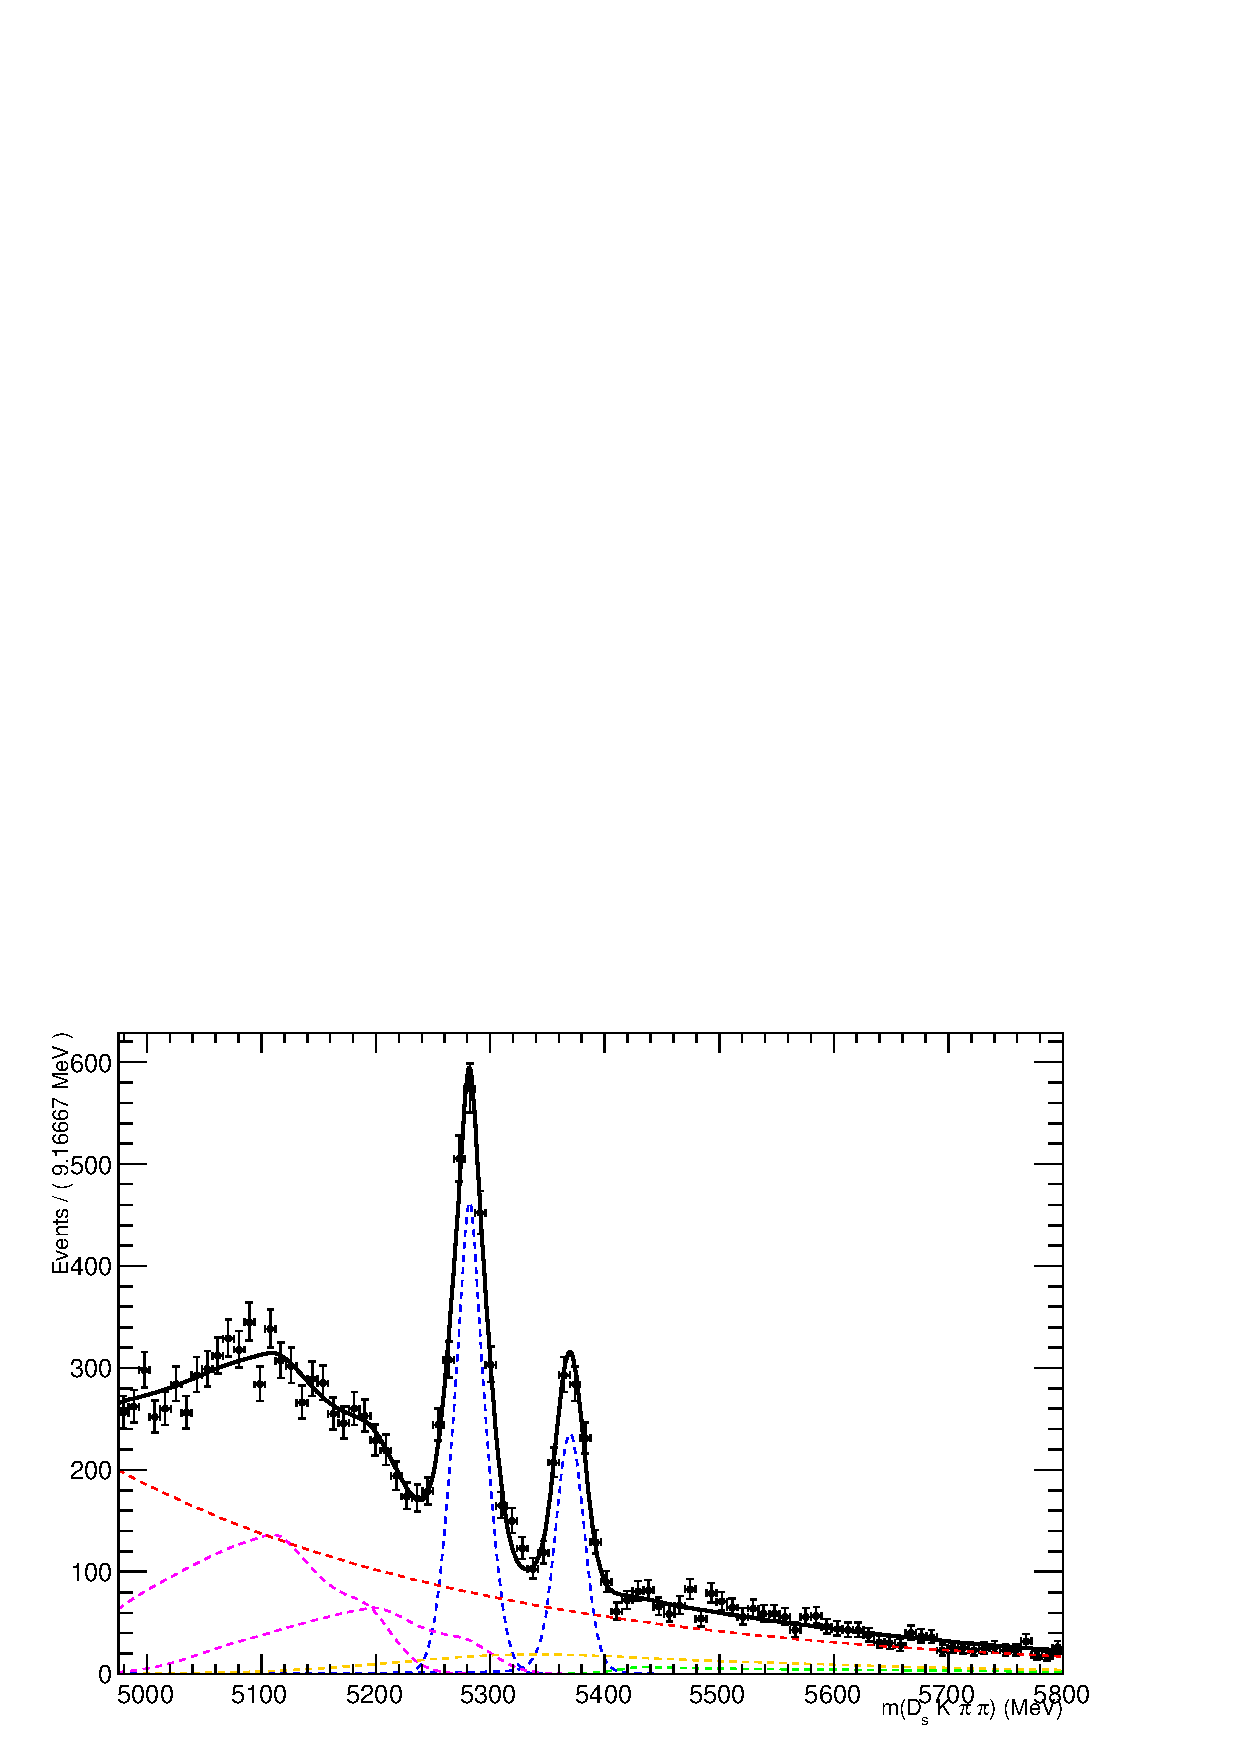
\includegraphics[width=0.5\textwidth, height = !]{plots/BmassFit_sim12.pdf} 	
	\end{figure}				
\end{frame}


\begin{frame}[plain]
%	\frametitle{TD Amplitude Analysis}

	\centering
	\vspace{-1cm}
		\includegraphics[width=0.49\textwidth, height = !]{plots/Bs_gamma.pdf} 	
		\includegraphics[width=0.49\textwidth, height = !]{plots/Bs_gamma_CP.pdf} 	
		
		
	\small
		\textbf{Full time-dependent amplitude PDF:}
		\scriptsize
	\begin{block}{}
\begin{align*}
	P(x,t,q_t,q_f) &\propto  [
	 \left( \vert A(x) \vert^2 + \vert \bar A(x) \vert^2 \right) \, \text{cosh} \left( \frac{\Delta \Gamma \, t}{2}\right) \\
	 & + q_t q_f \left( \vert A(x) \vert^2 - \vert \bar A(x) \vert^2 \right) \, \text{cos} \left( \Delta m_s \, t \right)  \\
	 & -2 \text{Re}\left( A(x)^{*}  \bar A(x) \, e^{-i q_f (\textcolor{red}{\gamma - 2\beta_s})}  \right) \, \text{sinh} \left( \frac{\Delta \Gamma \, t}{2}\right)  \\
	 & -2 q_t q_f \text{Im}\left( A(x)^{*}  \bar A(x) \, e^{-i q_f (\textcolor{red}{\gamma - 2\beta_s})}  \right)\, \text{sin} \left( \Delta  m_s \, t \right)  ]  e^{- \Gamma t}
\end{align*}
	\end{block}
%\newline
%\\

%	\small
$q_t = +1,0,-1$ for a $B_s^{0}$, no-,  ($\bar B_s^{0}$) tag  \\ 
$q_f$ = +1 $ $(-1) for $D_s^{-} K^{+} \pi\pi$ ($D_s^{+} K^{-} \pi\pi$) final states. 
				
\end{frame}


\begin{frame}
	\frametitle{Amplitude Analysis}

	\centering
	\small
	\textbf{Phasespace-integrated PDF:}
	\scriptsize
%Integrating over the phasespace, we get
	\begin{block}{}
\begin{align*}
	\int P(x,t,q_t,q_f) \text d x &\propto   [
	\, \text{cosh} \left( \frac{\Delta \Gamma \, t}{2}\right) \\
	 & + q_t q_f \left( \frac{1-r^2}{1+r^2} \right) \, \text{cos} \left( m_s \, t \right)  \\
	 & -2 \left( \frac{\kappa \, r \, \text{cos}(\delta - q_f(\gamma - 2 \beta_s))}{1+r^2}  \right) \, \text{sinh} \left( \frac{\Delta \Gamma \, t}{2}\right)  \\
	 & -2 q_t q_f \left( \frac{\kappa \, r \, \text{sin}(\delta - q_f(\gamma - 2 \beta_s))}{1+r^2}   \right)\, \text{sin} \left( m_s \, t \right)  ]  e^{- \Gamma t} \\
	 &=   [
	\, \text{cosh} \left( \frac{\Delta \Gamma \, t}{2}\right) 
	  + q_t q_f \, \textbf{C} \, \text{cos} \left( m_s \, t \right)   \\
	  & - \textcolor{red}{\kappa} \, \textbf{D}_{q_f} \, \text{sinh} \left( \frac{\Delta \Gamma \, t}{2}\right)  
	  - q_t \, \textcolor{red}{\kappa} \, \textbf{S}_{q_f}\, \text{sin} \left( m_s \, t \right)  ]  e^{- \Gamma t}
\end{align*}
	\end{block}
%where the $C,D_{q_f},S_{q_f}$ are defined exactly as for $D_s K$.
%The coherence factor is defined as :
%\begin{align*}
\vspace{0.2cm}
\small
$r \equiv \, \frac{\sqrt{\int \vert \bar A(x) \vert^2\text d x }}{\sqrt{\int \vert A(x) \vert^2\text d x}} $, 
$	\kappa \, e^{i\delta} \equiv \, \frac{\int A(x)^{*}  \bar A(x)  \text d x}{\sqrt{\int \vert A(x) \vert^2\text d x} \sqrt{\int \vert \bar A(x) \vert^2\text d x}  }$ %\end{align*}

\end{frame}


\begin{frame}
	\frametitle{Amplitude Analysis}

	\centering
		\small
	\textbf{Time-integrated, flavor averaged PDF:}
	
		\scriptsize

\begin{block}{}
\begin{align*}
	\int P(x,t,q_t,q_f) \, \text d t \, \text d q_t \, \text d q_f &\propto   \left( \vert A(x) \vert^2 + \vert \bar A(x) \vert^2 \right) \equiv \vert A^{eff}(x) \vert^2
\end{align*}
\end{block}

	\begin{block}{}
	\begin{itemize}
		\item No sensitivity to $\gamma$
		\item Useful to identify contributing amplitude components
	\end{itemize}
	\end{block}	

\end{frame}



%\begin{frame}
%	\frametitle{Sensitivity study}
%
%	\centering
%	
%	\begin{block}{Strategy}
%	\begin{itemize}
%		\item Time-integrated, flavor averaged fit: \\ $\Rightarrow$ Identify contributing amplitude components
%		\item Can we constrain coherence factor ?
%		\item Sensitivity on $\gamma$ depending on coherence factor
%	\end{itemize}
%	\end{block}	
%			
%\end{frame}

\begin{frame}
	\frametitle{Time-integrated, flavor averaged fit}

	\centering
	
	\begin{block}{}
	\begin{itemize}
		\item MINT2 fitter, used for $D \rightarrow 4 \pi$ [JHEP05(2017)143]
		\item Amplitude for $eg$ $B_s \to Ds^{-} \, ( K_1(1270)^{+} \to K^{+} \, \rho )$: 
		\\ $A^{eff}_i(x) = BW_{K_1}(m^{2}_{K\pi\pi}) \, BW_{\rho}(m^2_{\pi\pi}) \,  S_f$
		\item Sum over intermediate state amplitudes: 
		\\ $A^{eff}(x) = \sum_i a^{eff}_i \, A^{eff}_i(x)$
	\end{itemize}
	\end{block}	
	
	\begin{block}{\textbf{Very preliminary} fit}
	\begin{itemize}
		\item Signal region data, assuming $f_{Bkg} = 0$
		\item Assuming flat efficiency ($\epsilon(x) = 1$)
%		\item No flavour tagging:
%		\\ $\Rightarrow PDF = \vert A \vert^2 + \vert \bar{A} \vert^2 $
		\item Just for illustration, don't take it too seriously !
	\end{itemize}
	\end{block}
				
\end{frame}


\begin{frame}
	\frametitle{Amplitude Fit: $B_s \to D_s K \pi \pi$}

	\centering
	
	\begin{figure}[hp]
	\centering
%		\includegraphics[width=0.35\textwidth, height = 3.cm]{plots/WithAmps__leg.eps} 
		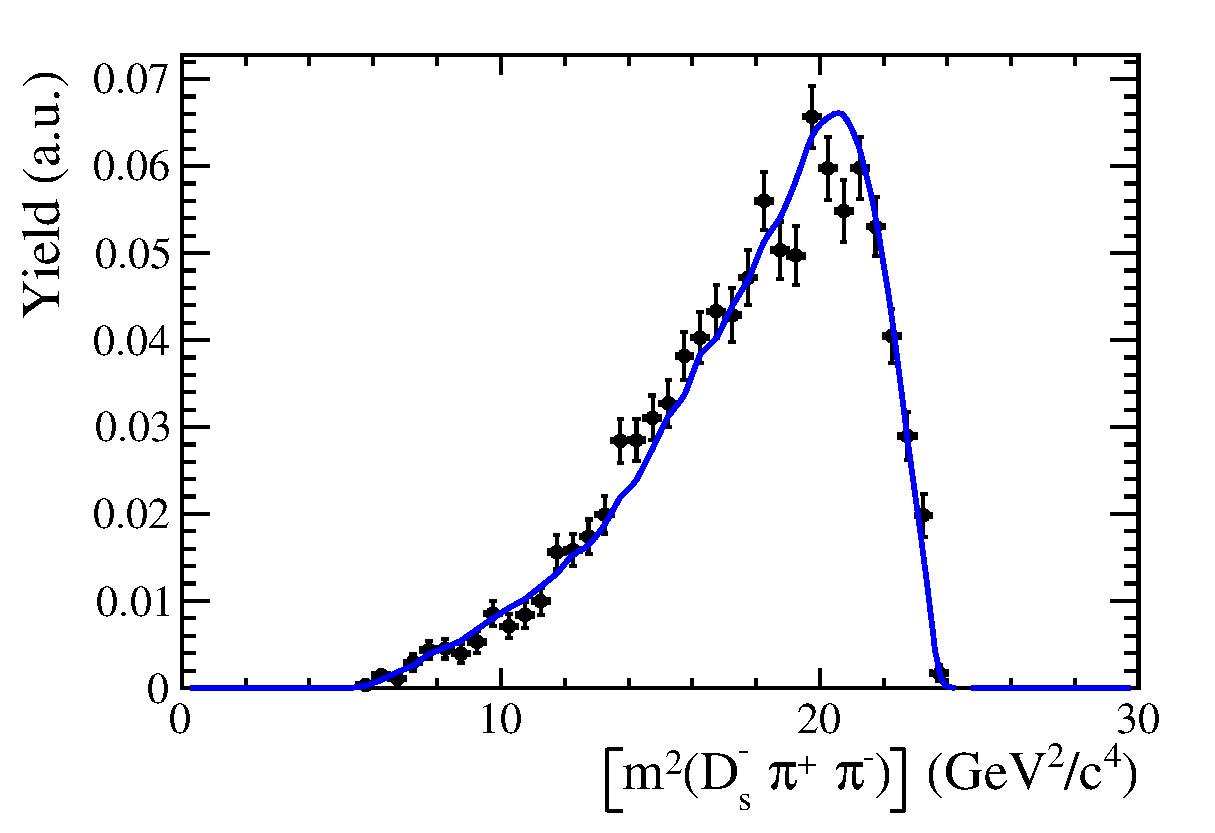
\includegraphics[width=0.35\textwidth, height = 3.cm]{plots/s_Dspipi.eps} 
		\includegraphics[width=0.35\textwidth, height = 3.cm]{plots/s_DsK.eps} 

		\includegraphics[width=0.35\textwidth, height = 3.cm]{plots/s_Kpipi.eps} 
		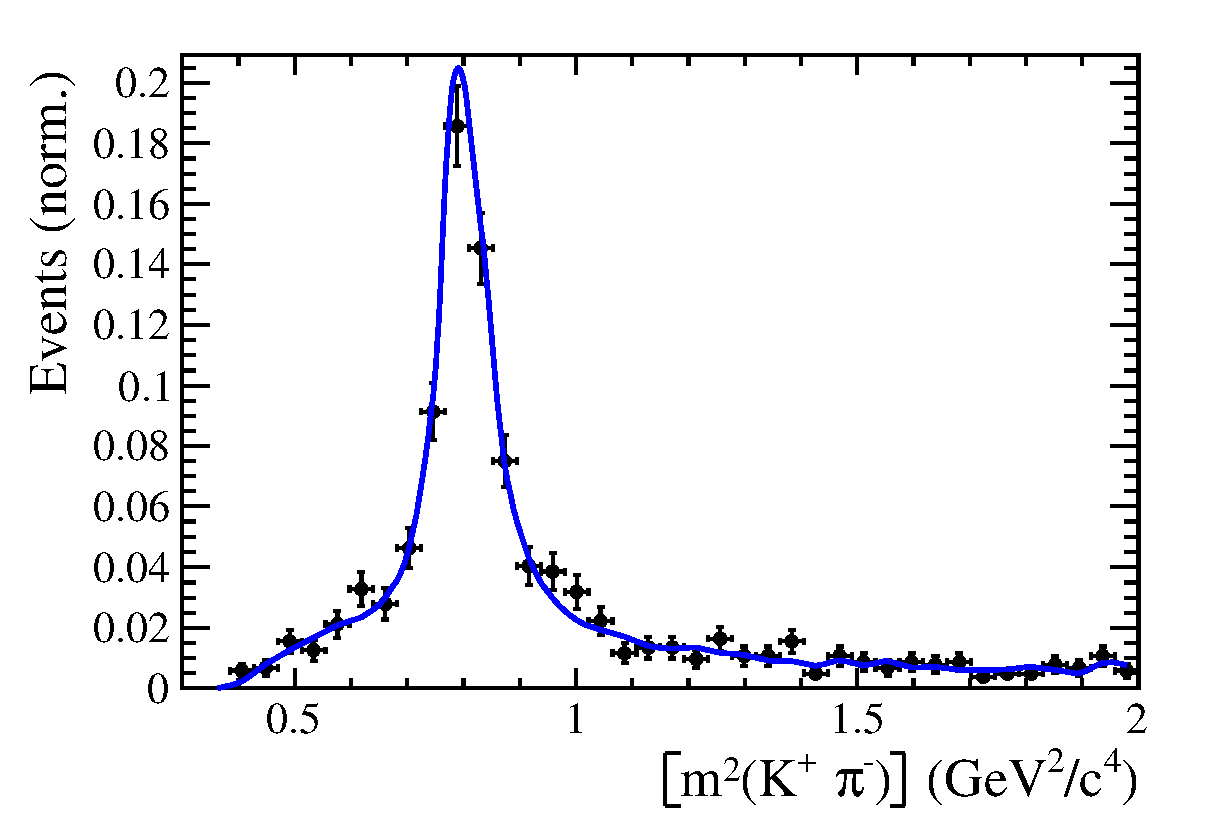
\includegraphics[width=0.35\textwidth, height = 3.cm]{plots/s_Kpi.eps} 
		\includegraphics[width=0.35\textwidth, height = 3.cm]{plots/s_pipi.eps} 		
	\end{figure}				
\end{frame}


\begin{frame}[fragile]
	\frametitle{Fit fractions}

	\centering
%      $F_i = \frac{\int ( \vert a_i  A_i(x) \vert^2 + \vert \bar a_i  \bar A_i(x) \vert^2 ) \, \text{d}x}{\int ( \vert A(x) \vert^2 + \vert\bar A(x) \vert^2 ) \, \text{d}x} $ \\
      $F^{eff}_i = \frac{\int  \vert a^{eff}_i  A^{eff}_i(x) \vert^2  \, \text{d}x}{\int  \vert A^{eff}(x) \vert^2 \, \text{d}x} $ \\


	\tiny
%	\centering
\begin{verbatim} 
	(1) Bs0->K(1)(1270)+(->K(0)*(1430)0(->K+,pi-),pi+),Ds- = 0.0520926 +/- 0.0145326
	(2) Bs0->K(1)(1270)+(->K*(892)0(->K+,pi-),pi+),Ds- = 0.090921 +/- 0.0214
	(3) Bs0->K(1)(1400)+(->K*(892)0(->K+,pi-),pi+),Ds- = 0.315657 +/- 0.0320033
	(4) Bs0->K*(1410)+(->K*(892)0(->K+,pi-),pi+),Ds- = 0.127998 +/- 0.0175661
	(5) Bs0->NonResS0(->Ds-,pi+),K*(892)0(->K+,pi-) = 0.0265594 +/- 0.0114541
	(6) Bs0[D]->NonResV0(->Ds-,pi+),K*(892)0(->K+,pi-) = 0.0108669 +/- 0.0069929
	(7) Bs0->NonResA0(->sigma10(->pi+,pi-),Ds-),K+ = 0.0715845 +/- 0.0247102
	(8) Bs0->NonResV0(->Ds-,K+),sigma10(->pi+,pi-) = 0.139525 +/- 0.0321404
	(9) Bs0->K(1)(1270)+(->rho(770)0(->pi+,pi-),K+),Ds- = 0.16488 +/- 0.0379784
	(10) Bs0->K(1)(1400)+(->rho(770)0(->pi+,pi-),K+),Ds- = 0.071005 +/- 0.0218139
	(11) Bs0->K*(1410)+(->rho(770)0(->pi+,pi-),K+),Ds- = 0.0766048 +/- 0.014699
	(12) Bs0->NonResA0(->rho(770)0(->pi+,pi-),Ds-),K+ = 0.0210193 +/- 0.0104696
	 sum = 1.16871 +/- 0.0595647(fit)
\end{verbatim}	
				
\end{frame}



%\begin{frame}
%	\frametitle{Coherence Factor}
%
%	\centering
%	
%	\begin{block}{}
%	\begin{itemize}
%		\item   $A(x) = \sum_i a_i \, A_i(x)$   \\
%		 $\bar A(x) = \sum_i \bar a_i \, \bar A_i(x)$
%		\item Use amplitudes from flavor-averaged, time-integrated fit
%		 \item Draw random $a_i$ and $\bar a_i $ values
%		 \item Constraints: \\
%		 $\int ( \vert a_i  A_i(x) \vert^2 + \vert \bar a_i  \bar A_i(x) \vert^2 ) \, \text{d}x / N = F^{eff}_i $ \\
%		 $r \approx 0.4 $ (ration of CKM elements)
%	\end{itemize}
%	\end{block}	
%	
%	\begin{figure}[hp]
%		\centering
%		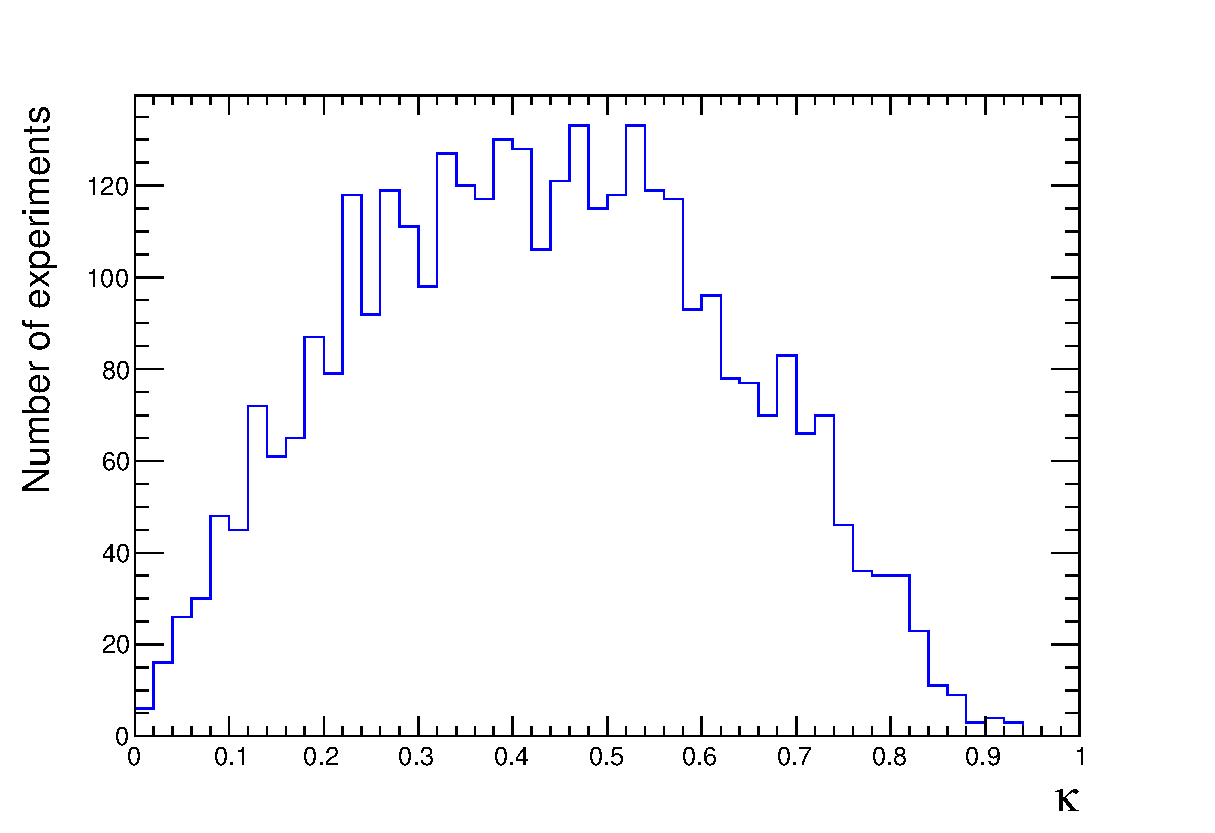
\includegraphics[width=0.45\textwidth, height = ! ]{plots/k.eps} 
%	\end{figure}				
%
%\end{frame}

%\begin{frame}
%	\frametitle{Coherence Factor}
%
%	\centering
%	
%	\begin{table}[h]
%  \footnotesize
%  \centering
%  \begin{tabular}
%    {l c c }
%    \hline \hline
%    Region &  $<\kappa> (\%)$   &  Cut eff. $(\%)$ \\   \hline
%    Full & 43 &  100 \\
%    $K^*(892)$ & 51    &  43  \\
%    $\rho^0(770)$ & 46  & 47   \\
%    $K_1(1270)$ & 61   & 23  \\
%%    Full & $43$ & 40 & 100 \\
%%    $K^*(892)$ & 51 &  42   &   \\
%%    $\rho^0(770)$ & 46  & 41  &   \\
%%    $K_1(1270)$ & 61   & 44   &   \\
%    \hline \hline
%  \end{tabular}
%  \label{tab:sideband}
%\end{table}
%	
%	\begin{figure}[hp]
%	\centering
%%		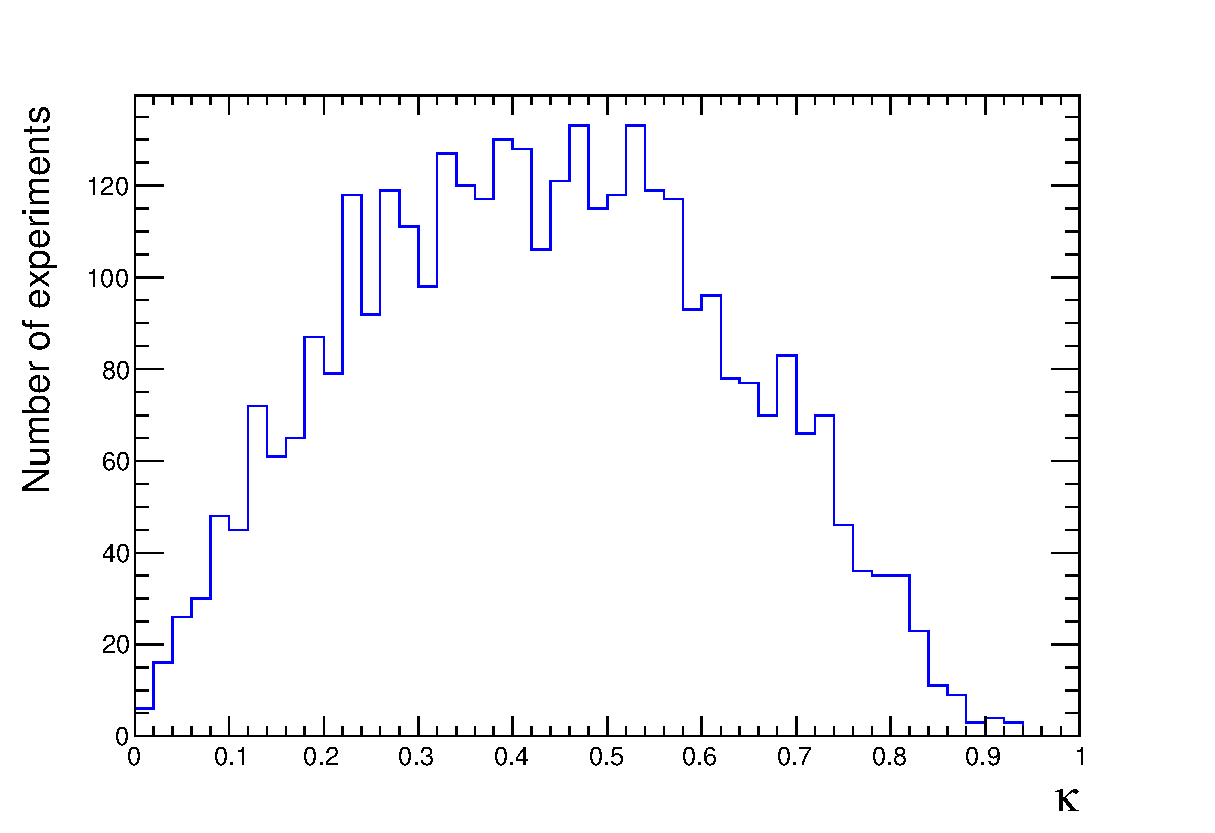
\includegraphics[width=0.35\textwidth, height = 3.cm]{plots/k.eps} 
%		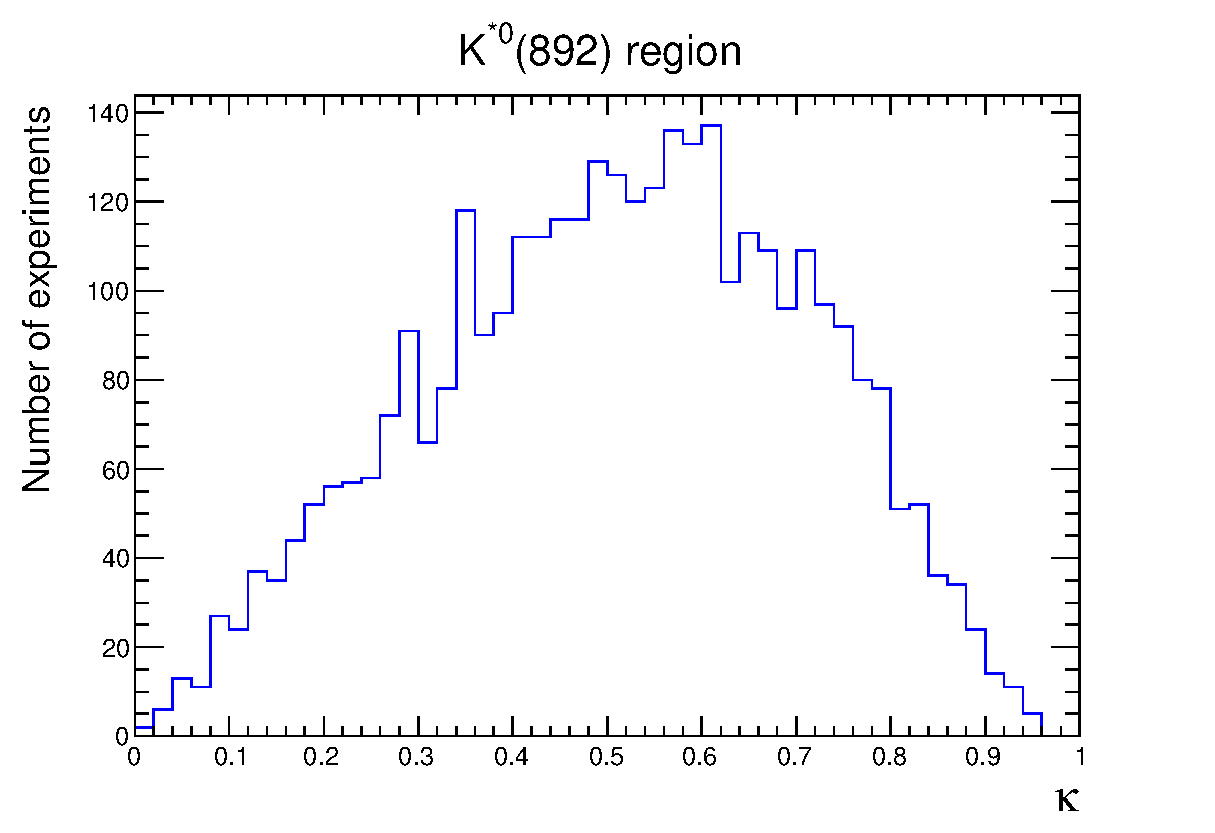
\includegraphics[width=0.35\textwidth, height = 3.cm]{plots/k_Ks.eps} 
%		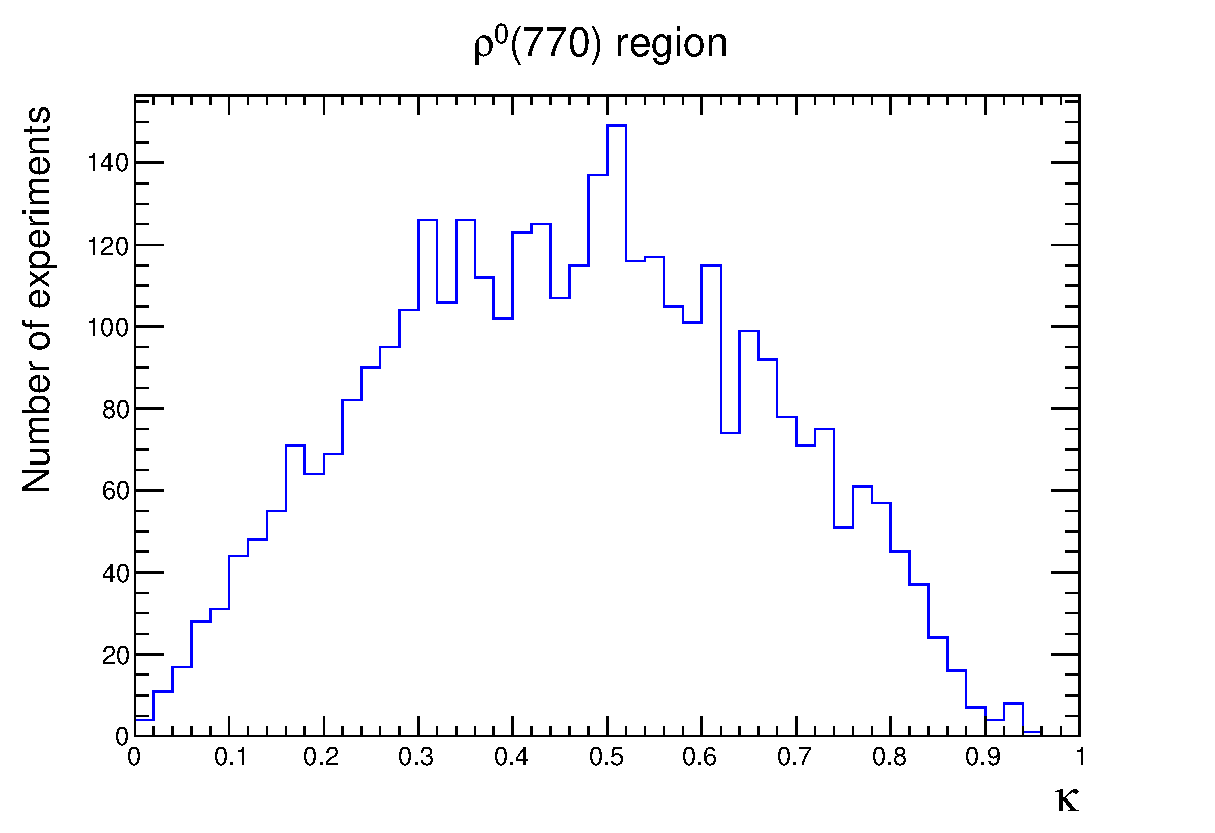
\includegraphics[width=0.35\textwidth, height = 3.cm]{plots/k_rho.eps} 
%		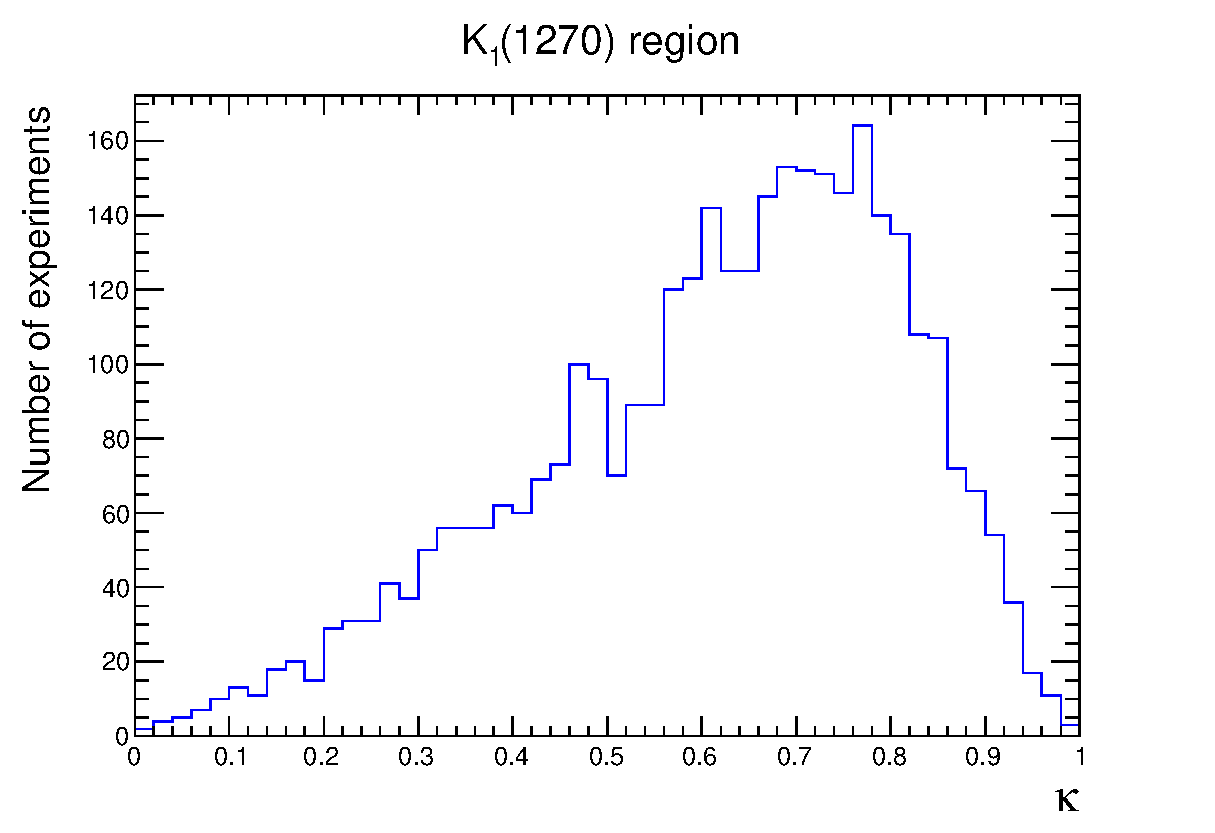
\includegraphics[width=0.35\textwidth, height = 3.cm]{plots/k_K1.eps} 		
%	\end{figure}				
%\end{frame}



\begin{frame}
	\frametitle{Sensitivity Studies}

	\centering
	
	\begin{block}{}
	\begin{itemize}
		\item  Developed time-dependent MINT extension
		\item Generate toys with different values for $\kappa$ 
		\item Compare sensitivity to $\gamma$ fitting with \\ \textbf{full PDF} and with \textbf{phasespace-integrated PDF}
		\end{itemize}
	\end{block}		
		
	\begin{block}{Assumptions}
	\begin{itemize}	
		\item Use amplitudes from flavor-averaged, time-integrated fit
		\item $r = 0.4$ (ratio of CKM elements) 
		\item PDG values for: $\tau,\Delta m_s, \Delta \Gamma, \beta_s$
		\item $\epsilon(x,t) = const.$, perfect resolution  
		\item $\epsilon_{Tag} = 0.66, <\omega> = 0.4 $   
		\item $N_{signal} = 3000$ (Run1+15/16 data)		 
	\end{itemize}
	\end{block}	
			

\end{frame}


\begin{frame}
	\frametitle{Example Toy-Fit: $B_s \to D_s K \pi \pi$}

	\centering
	
	\begin{figure}[hp]
	\centering
		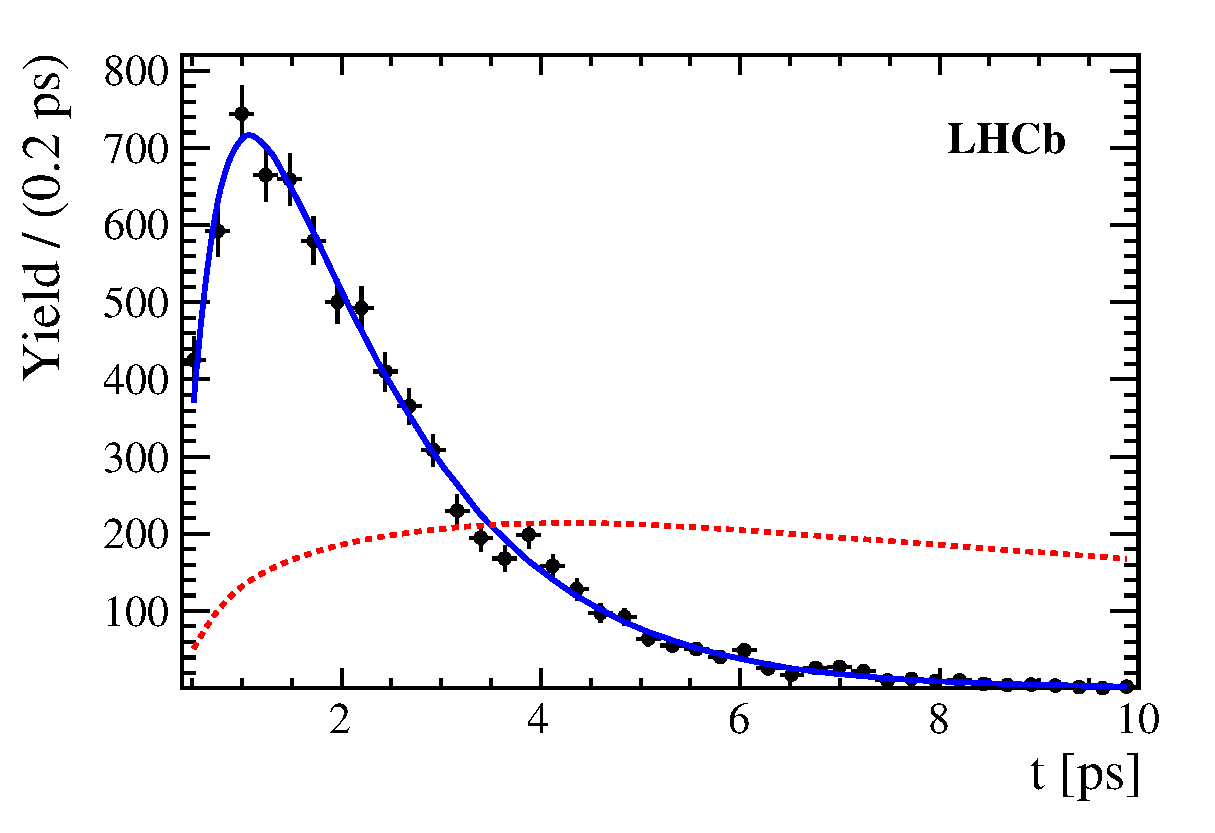
\includegraphics[width=0.35\textwidth, height = 3.cm]{plots_toy/h_t.eps} 
		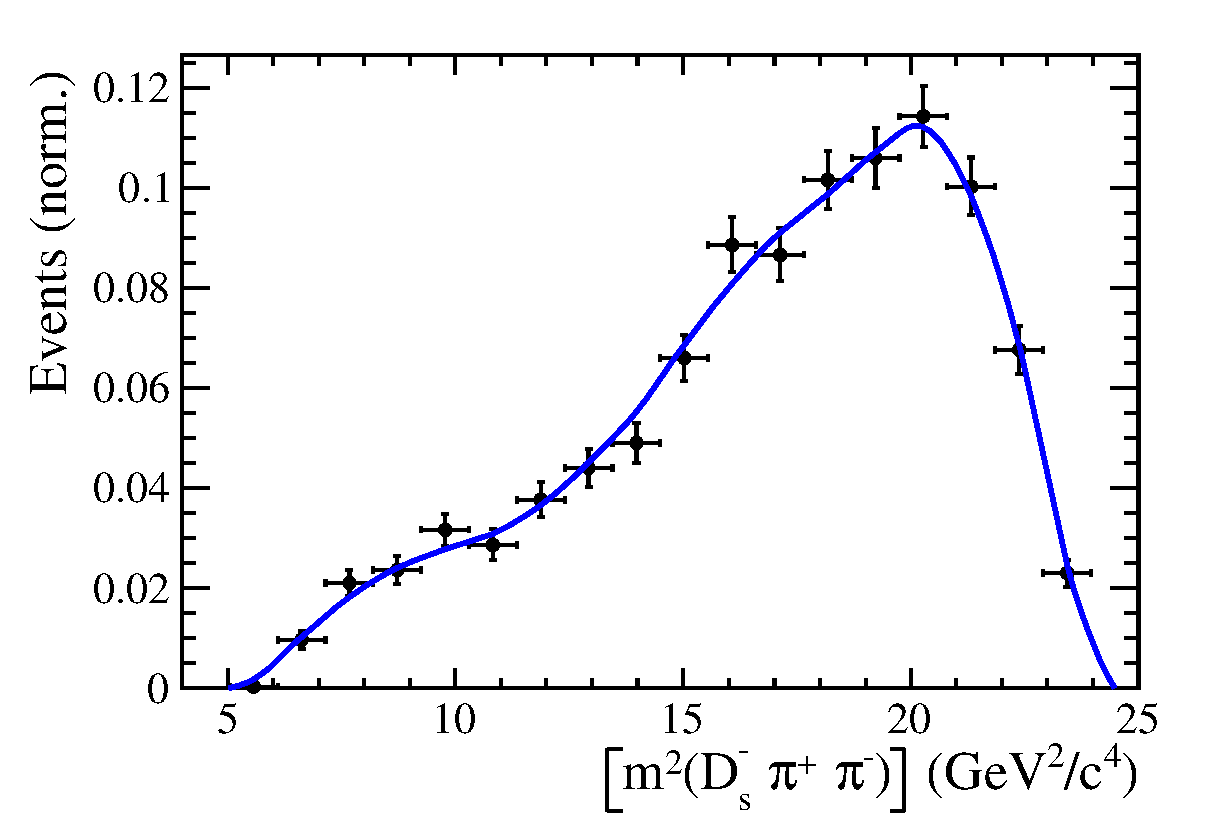
\includegraphics[width=0.35\textwidth, height = 3.cm]{plots_toy/s_Dspipi.eps} 
		\includegraphics[width=0.35\textwidth, height = 3.cm]{plots_toy/s_DsK.eps} 

		\includegraphics[width=0.35\textwidth, height = 3.cm]{plots_toy/s_Kpipi.eps} 
		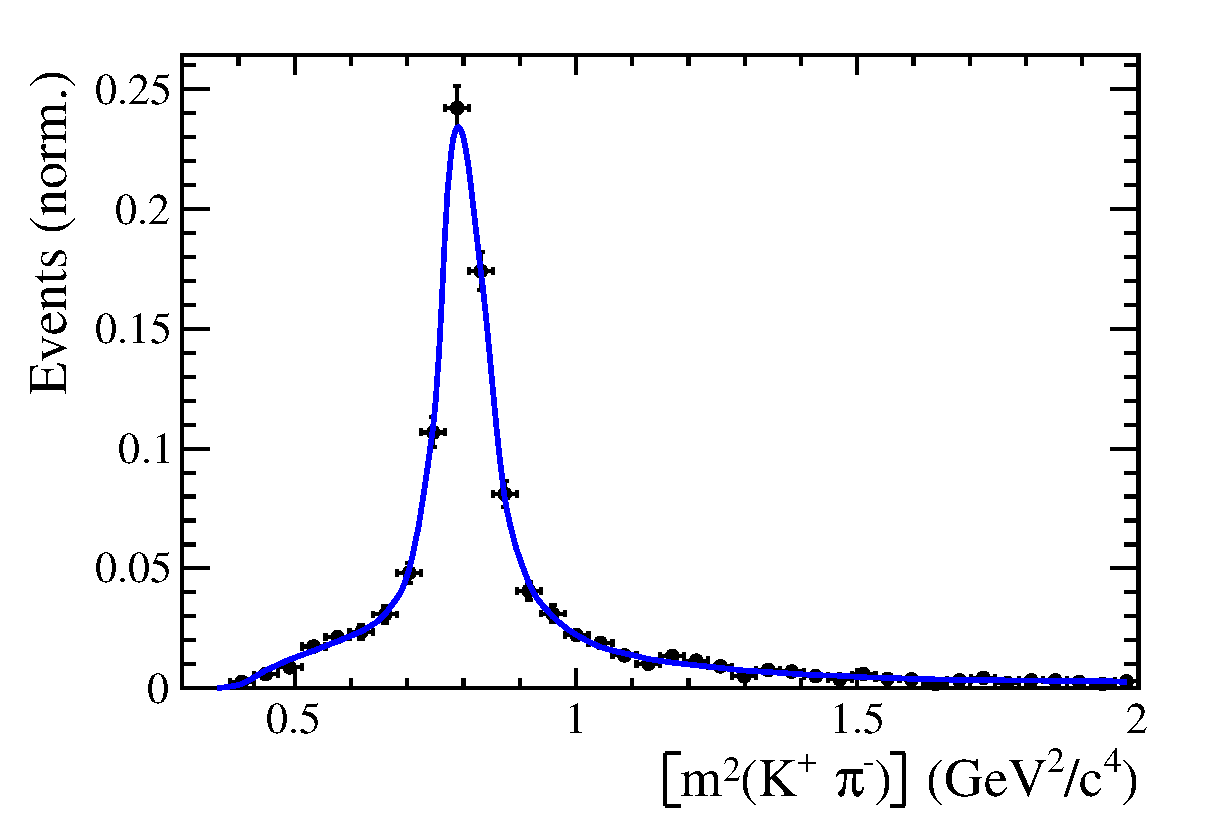
\includegraphics[width=0.35\textwidth, height = 3.cm]{plots_toy/s_Kpi.eps} 
		\includegraphics[width=0.35\textwidth, height = 3.cm]{plots_toy/s_pipi.eps} 		
	\end{figure}				
\end{frame}

\begin{frame}
	\frametitle{Example Toy-Fit: $B_s \to D_s K \pi \pi$}

	\centering
	
	\begin{block}{}
	\begin{itemize}
		\item  \textcolor{red}{$B_s (\bar B_s) \to D_s^- K^+ \pi \pi$}
		 \item  \textcolor{blue}{$B_s (\bar B_s) \to D_s^+ K^- \pi \pi$}
		\item  \textcolor{green}{$Untagged \to D_s^- K^+ \pi \pi \, (D_s^+ K^- \pi \pi)$}

	\end{itemize}
	\end{block}	
	
	\begin{figure}[hp]
	\centering
		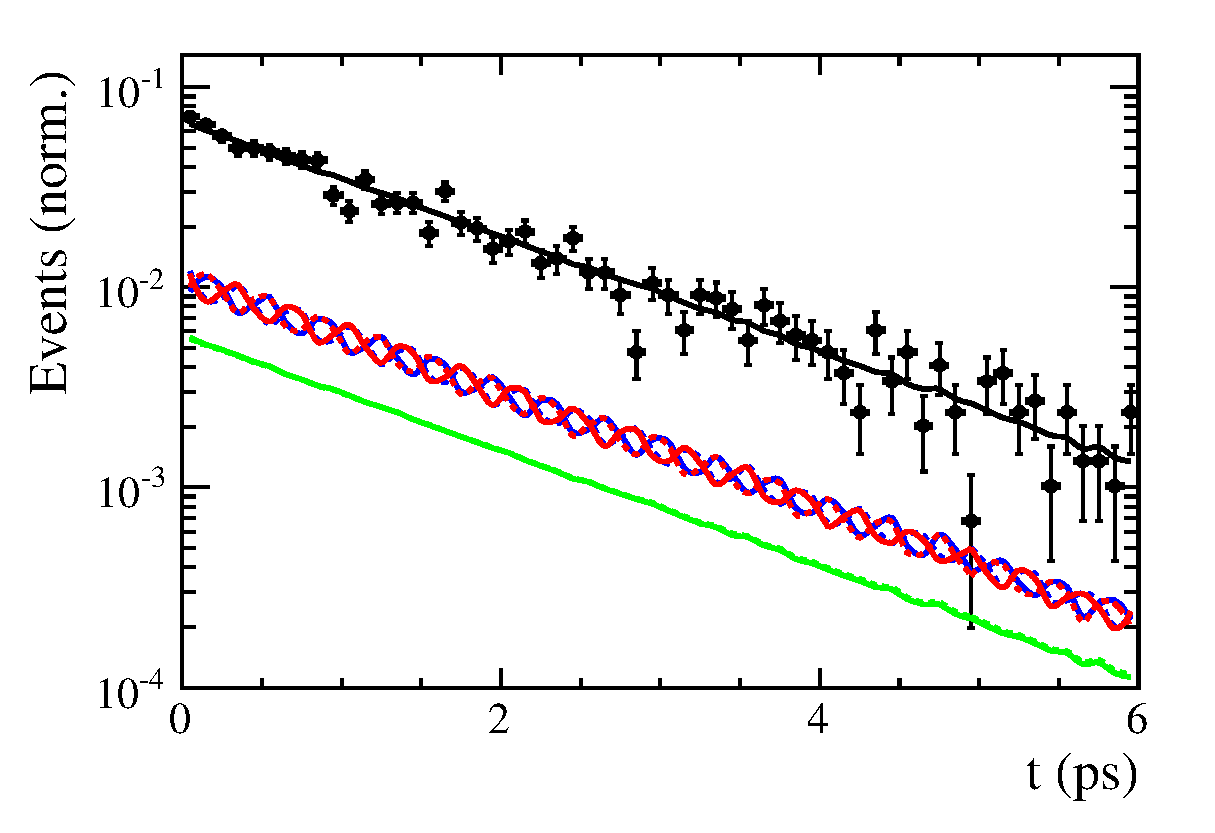
\includegraphics[width=0.5\textwidth, height = !]{plots_toy/h_t_2_log.eps} 		
	\end{figure}				
\end{frame}

\begin{frame}
	\frametitle{Likelihood Scan}

	\centering
	
	\begin{figure}[hp]
	\centering
		
		$D_s^+ K^- \pi \pi$      \hspace{2cm}     $D_s^- K^+ \pi \pi$   \hspace{2cm}   Combined
		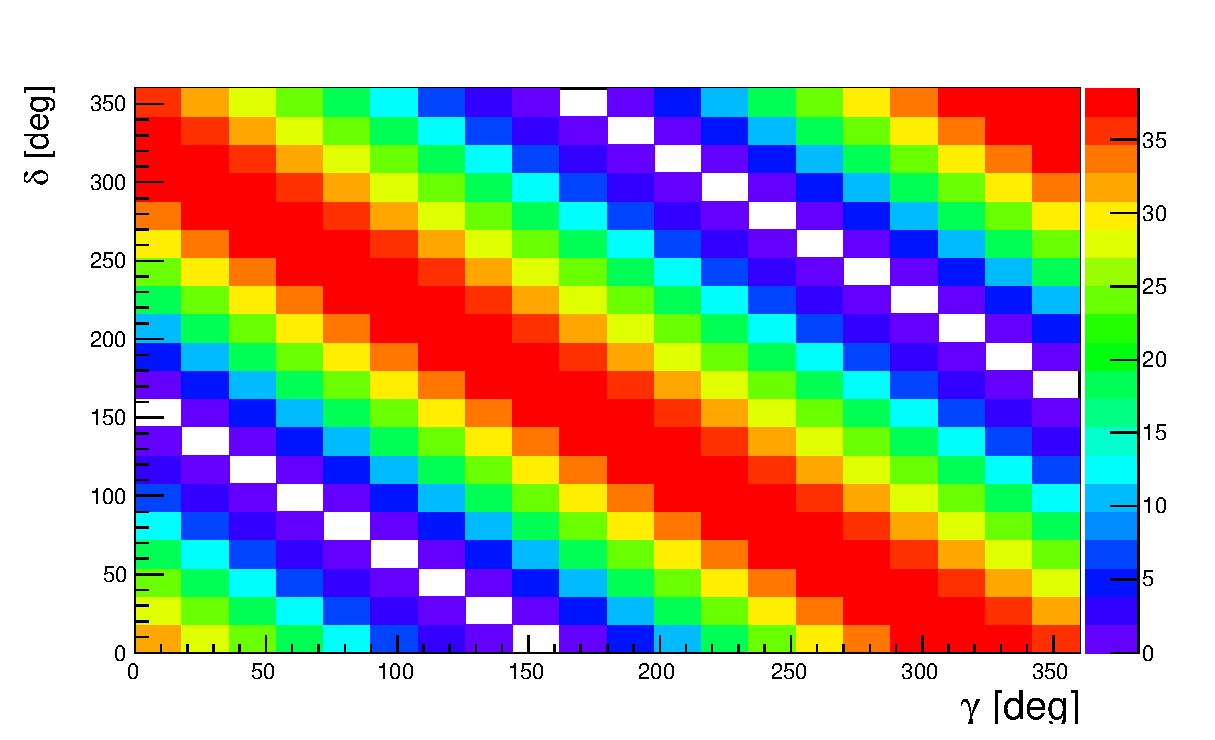
\includegraphics[width=0.35\textwidth, height = 3.cm]{plots/LL_scan_m.eps} 
		\includegraphics[width=0.35\textwidth, height = 3.cm]{plots/LL_scan_p.eps} 
		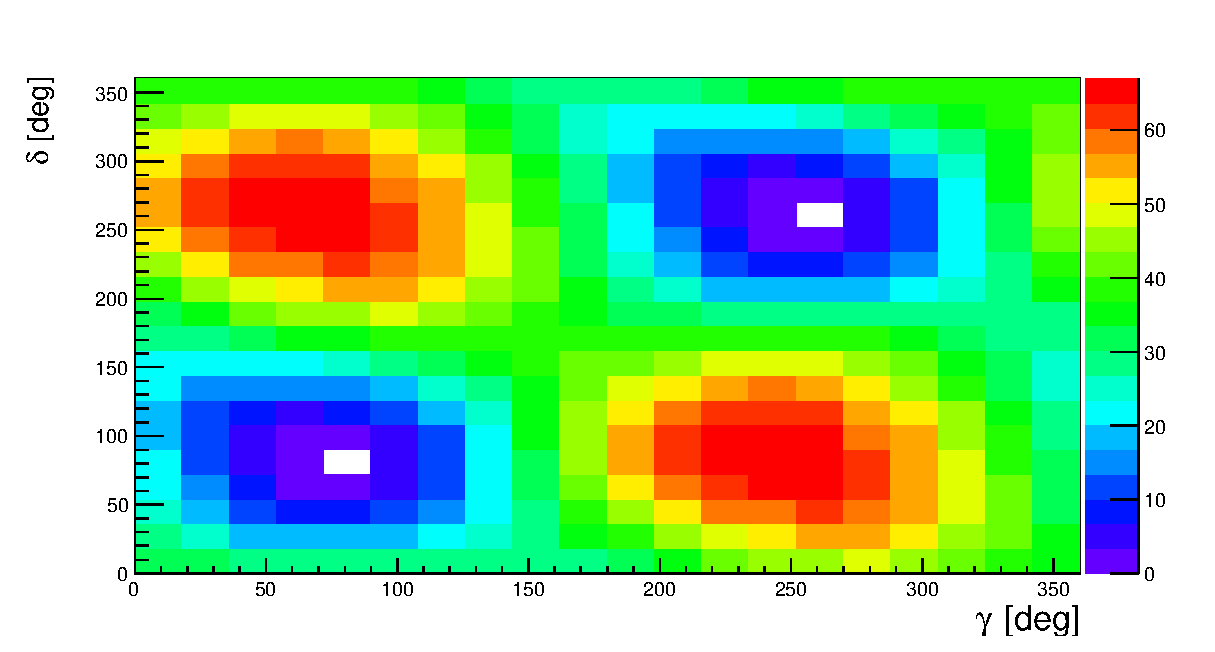
\includegraphics[width=0.35\textwidth, height = 3.cm]{plots/LL_scan.eps} 
		
		Generated values: \\  $\gamma = 70^{\circ}, \delta = 100^{\circ}$ \\
		Fit result:    \\ $\gamma = 74 \pm 15^{\circ}, \delta = 84 \pm 15^{\circ}$ \\
		 ($\gamma = 254 \pm 15^{\circ}, \delta = 264 \pm 15^{\circ}$)

		
	\end{figure}		
				
\end{frame}

\begin{frame}
	\frametitle{Fit Validation}

	\centering
	
	\begin{figure}[hp]
	\centering
		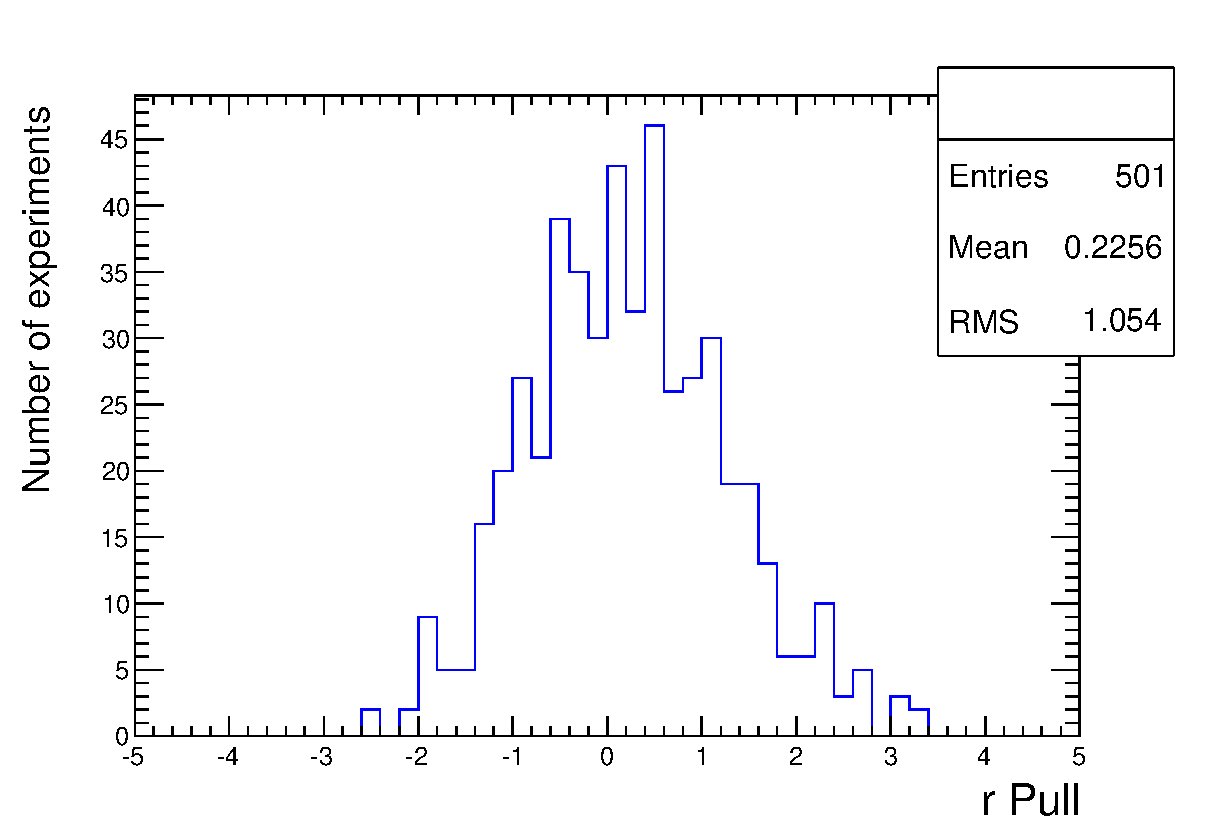
\includegraphics[width=0.4\textwidth, height = 3.cm]{plots_toy/r_pull.eps} 
		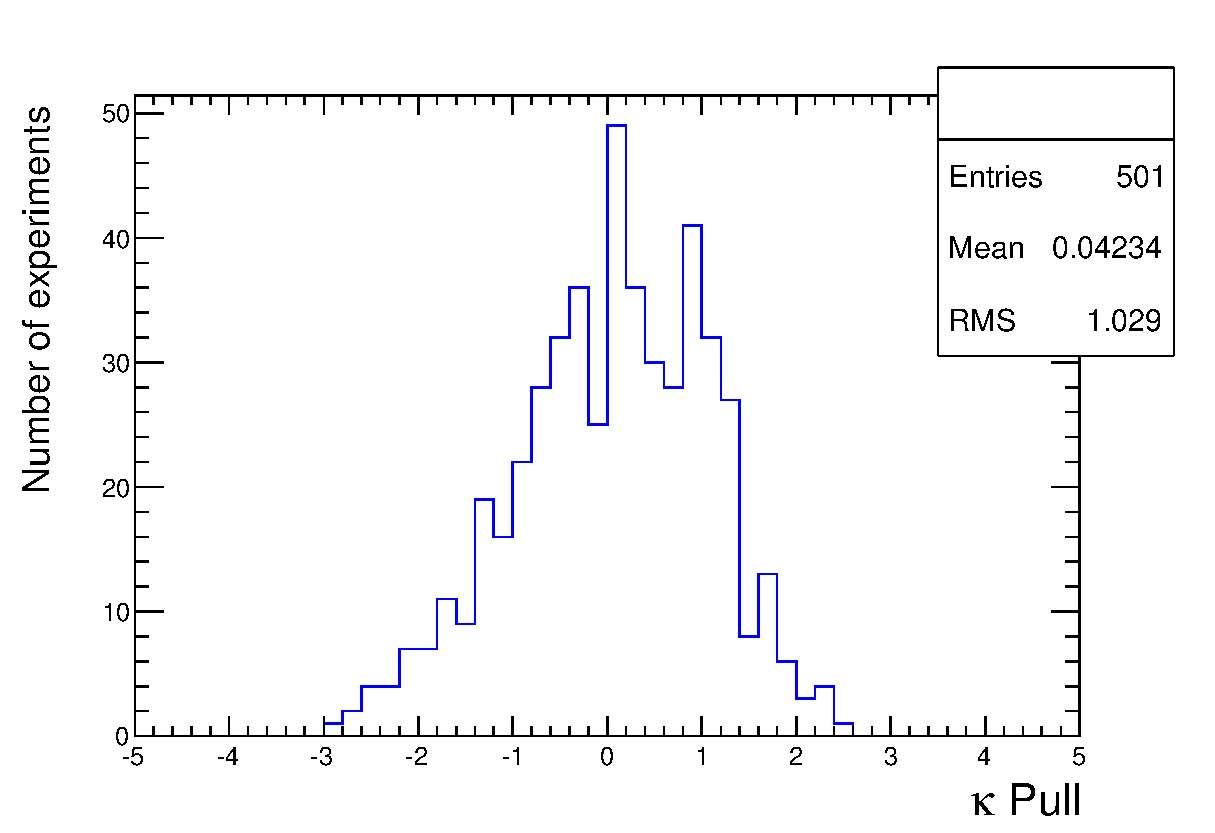
\includegraphics[width=0.4\textwidth, height = 3.cm]{plots_toy/k_pull.eps} 
		
		\includegraphics[width=0.4\textwidth, height = 3.cm]{plots_toy/gamma_pull.eps} 
		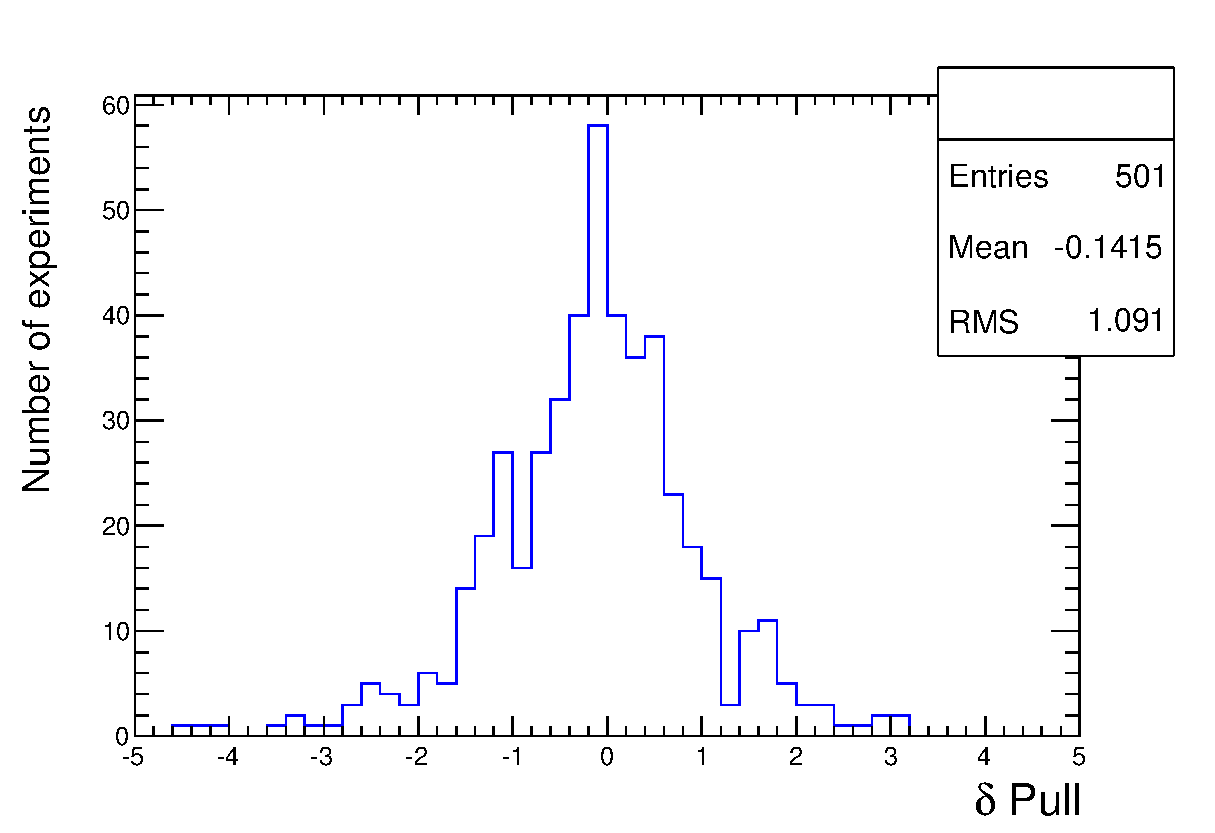
\includegraphics[width=0.4\textwidth, height = 3.cm]{plots_toy/delta_pull.eps} 

		
	\end{figure}		
				
\end{frame}


\begin{frame}[plain]
%	\frametitle{Sensitivity Study}

	\centering	
	\begin{table}[h]
  \scriptsize
  \centering
  \begin{tabular}
    {l c c c c}
    \hline \hline
    & Generated &  Full PDF     &   Phasespace integrated  \\   \hline
	$r$ & 0.4 & $0.38 \pm 0.06$   &  unstable \\
	$\kappa$  & \textcolor{red}{0.2} & $0.23 \pm 0.13$ & 0.2 (fixed)  \\
	$\delta$ & 100 & $99 \pm 22$ &  unstable\\
	$\gamma$ & 70 & $70 \pm 17$  & unstable \\
    \hline \hline
  \end{tabular}
\end{table}

	\begin{table}[h]
  \scriptsize
  \centering
  \begin{tabular}
    {l c c c c}
    \hline \hline
    & Generated &  Full PDF    &   Phasespace integrated  \\   \hline
	$r$ & 0.4 & $0.44 \pm 0.07$      & $0.43 \pm 0.11$  \\
	$\kappa$  & \textcolor{red}{0.4} &$0.41 \pm 0.14$  & 0.4 (fixed)  \\
	$\delta$ & 100 & $101 \pm 19$  & $95 \pm 41$ \\
	$\gamma$ & 70 & $69 \pm 16$   & $66 \pm 40 $ \\
    \hline \hline
  \end{tabular}
\end{table}

	\begin{table}[h]
  \scriptsize
  \centering
  \begin{tabular}
    {l c c c c}
    \hline \hline
    & Generated &  Full PDF    &   Phasespace integrated  \\   \hline
	$r$ & 0.4 & $0.41 \pm 0.08$     & $0.39 \pm 0.11$  \\
	$\kappa$  & \textcolor{red}{0.6} & $0.60 \pm 0.13$  & 0.6 (fixed)  \\
	$\delta$ & 100 & $98 \pm 17$ & $92 \pm 25$ \\
	$\gamma$ & 70 & $68 \pm 17$ & $65 \pm 28$ \\
    \hline \hline
  \end{tabular}
\end{table}

	\begin{table}[h]
  \scriptsize
  \centering
  \begin{tabular}
    {l c c c c}
    \hline \hline
    & Generated &  Full PDF        &   Phasespace integrated  \\   \hline
	$r$ & 0.4 & $0.42 \pm 0.09$    &  $0.39 \pm 0.09$ \\
	$\kappa$  & \textcolor{red}{1.0} & $0.96 \pm 0.03$ &  1.0 (fixed)  \\
	$\delta$ & 100 & $100 \pm 17$ &  $100 \pm 17$  \\
	$\gamma$ & 70 & $66 \pm 17$ & $67 \pm 17$  \\
    \hline \hline
  \end{tabular}
\end{table}

\end{frame}
	

%\begin{frame}
%	\frametitle{Amplitude Fit: $B_s \to D_s \pi \pi \pi$}
%
%	\centering
%	
%	\begin{figure}[hp]
%	\centering
%	
%%		\includegraphics[width=0.35\textwidth, height = 3.cm]{BsDs3pi/WithAmps__leg.eps} 
%		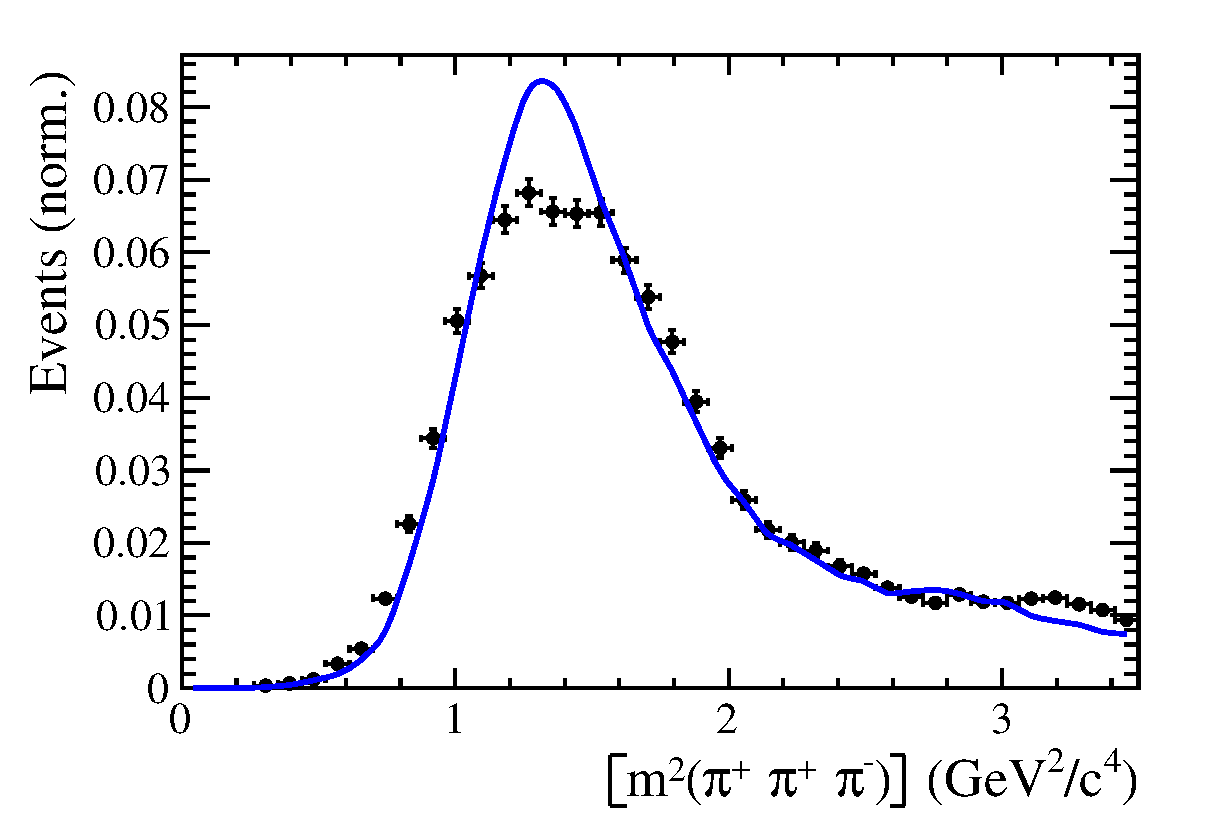
\includegraphics[width=0.35\textwidth, height = 3.cm]{BsDs3pi/s_pipipi.eps} 
%		\includegraphics[width=0.35\textwidth, height = 3.cm]{BsDs3pi/s_pipi.eps} 		
%		
%		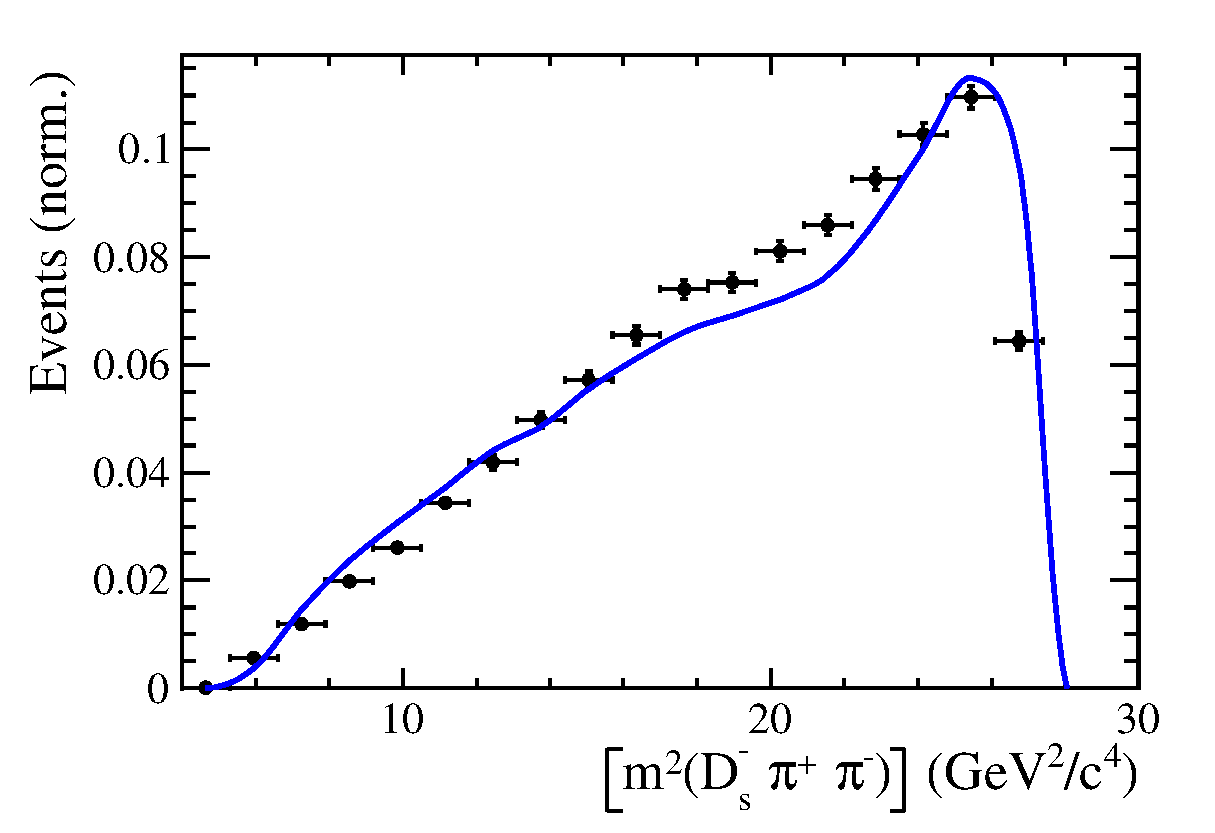
\includegraphics[width=0.35\textwidth, height = 3.cm]{BsDs3pi/s_Dspipi.eps} 
%		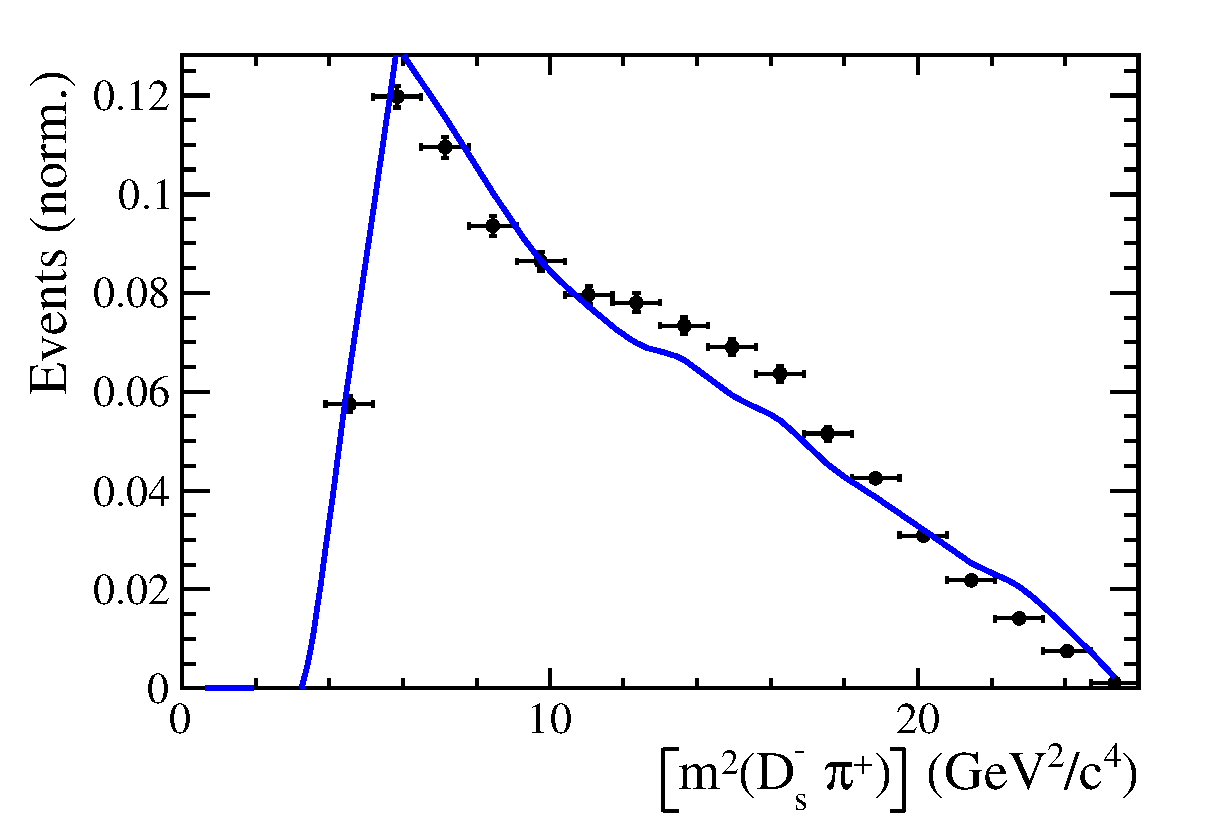
\includegraphics[width=0.35\textwidth, height = 3.cm]{BsDs3pi/s_Dspi.eps} 
%		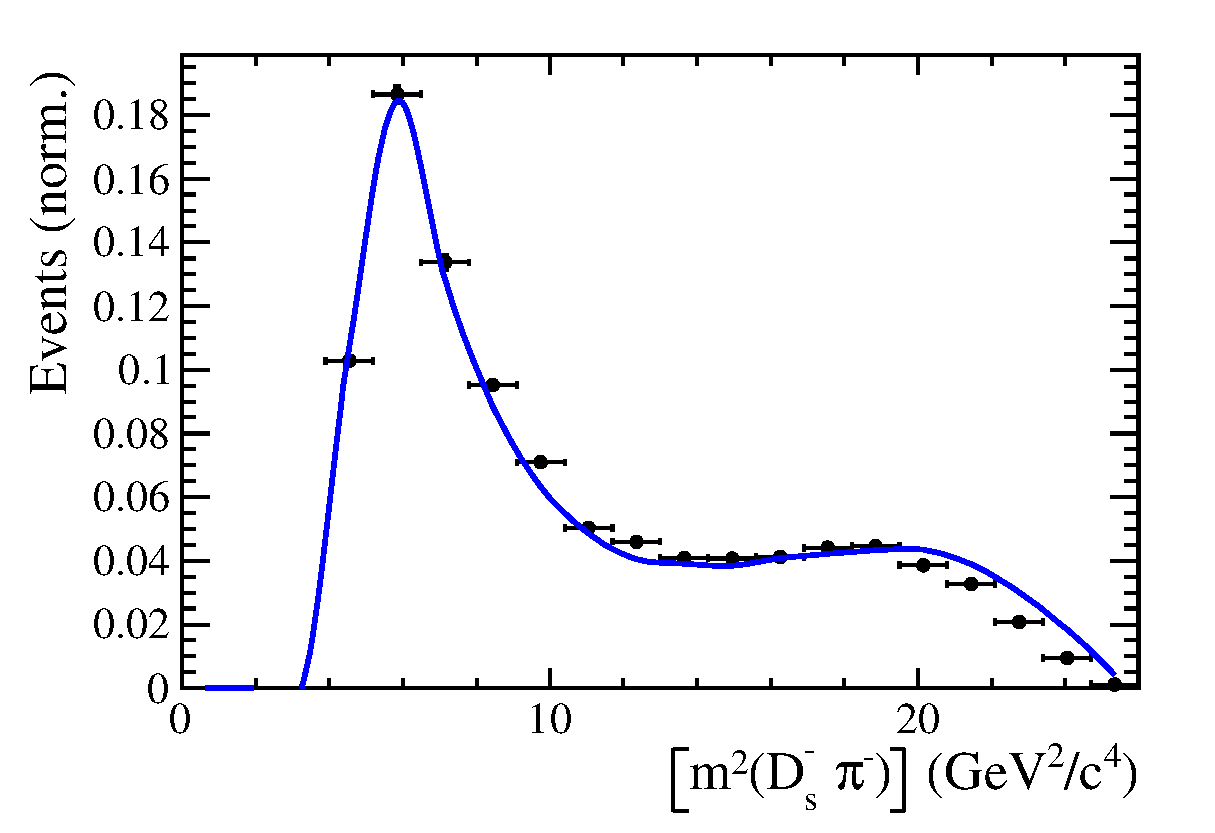
\includegraphics[width=0.35\textwidth, height = 3.cm]{BsDs3pi/s_Dspi_2.eps} 
%
%		
%	\end{figure}		
%				
%\end{frame}
%
%\begin{frame}[fragile]
%	\frametitle{Fit fractions}
%
%	\tiny
%%	\centering
%\begin{verbatim} 
%	(1) Bs0->f(0)(1370)0(->pi+,pi-),NonResS0(->Ds-,pi+) = 0.0302852 +/- 0.00196946
%	(2) Bs0->NonResS0(->Ds-,pi+),sigma10(->pi+,pi-) = 0.0279803 +/- 0.00266628
%	(3) Bs0->a(1)(1260)+(->sigma10(->pi+,pi-),pi+),Ds- = 0.118991 +/- 0.00456337
%	(4) Bs0->NonResV0(->Ds-,pi+),rho(770)0(->pi+,pi-) = 0.175701 +/- 0.00692438
%	(5) Bs0->a(1)(1260)+(->rho(770)0(->pi+,pi-),pi+),Ds- = 0.427705 +/- 0.00741986
%	(6) Bs0->a(1)(1640)+[D](->rho(770)0(->pi+,pi-),pi+),Ds- = 0.0115973 +/- 0.00131729
%	(7) Bs0[D]->NonResV0(->Ds-,pi+),rho(770)0(->pi+,pi-) = 0.1135 +/- 0.00509339
%==========================================================
%	 sum = 0.908828 +/- 0.0103227(fit) +/- 0.00150787(integ)
%\end{verbatim}	
%				
%\end{frame}
%
%\begin{frame}
%	\frametitle{Conclusion}
%	
%	\begin{block}{$B_s \to D_s \pi \pi \pi$}
%	\begin{itemize}
%		\item Dominated by $B_s \to D_s \, a_1(1260)$
%		\item Interesting channel for spectroscopy: \\Search for $(D_s \pi \pi)$, $(D_s \pi)$ resonances
%		\item High statistics, no flavor tagging needed, can be done time-integrated
%		\item Could also measure $\Delta m_s, \Delta \Gamma$
%		\item Will not be pursued further ... 
%	\end{itemize}
%	\end{block}
%	
%\end{frame}

\begin{frame}
	\frametitle{Conclusion}
	
	\begin{block}{$B_s \to D_s K \pi \pi$}
	\begin{itemize}
		\item \textbf{Estimated sensitivity to $\gamma$:}\\ 
		 $17^{\circ}$ independent of $\kappa$ using TD-amplitude fit \\
		  $17^{\circ}$ ($40^{\circ}$) for $\kappa = 1$ ($\kappa = 0.4$) using phasespace-integrated fit
%		\item Dominated by $B_s \to D_s \, K_1(1270)$
%		\item \textbf{Coherence factor:} 
%		\\ Not worth to select a resonance to enhance coherence
%		\\ Need TD-amplitude fit to estimate it
		\item \textbf{ToDo:}
%		\\ Flavor tagging
		\\ Reimplement time-acceptance/resolution from \\ B2DX-Fitter in MINT
	\end{itemize}
		\end{block}

\end{frame}


\end{document}